% Share of eligible MSCA applicants who applied to the Global rather than the European
% Fellowship, by panel, 2016-2025. GENERATED BY msca_figures.py - edit that file, not this one.
% Eligible proposals (EF/GF): SOC 2016:1456/221 2017:1511/232 2018:1637/247 2019:1740/316 2020:2105/396 2021:1624/344 2022:1387/285 2023:1580/397 2024:1912/436 2025:3208/530; ECO 2016:197/26 2017:178/21 2018:152/23 2019:168/11 2020:175/16 2021:123/9 2022:109/11 2023:121/8 2024:162/15 2025:246/15; CHE 2016:940/65 2017:1012/71 2018:1056/62 2019:1061/58 2020:1230/62 2021:1062/65 2022:920/42 2023:1074/57 2024:1428/60 2025:2360/67
\definecolor{mscaSOC}{HTML}{2A78D6}
\definecolor{mscaECO}{HTML}{EB6834}
\definecolor{mscaCHE}{HTML}{1BAF7A}
\begin{figure}[htbp]
\centering
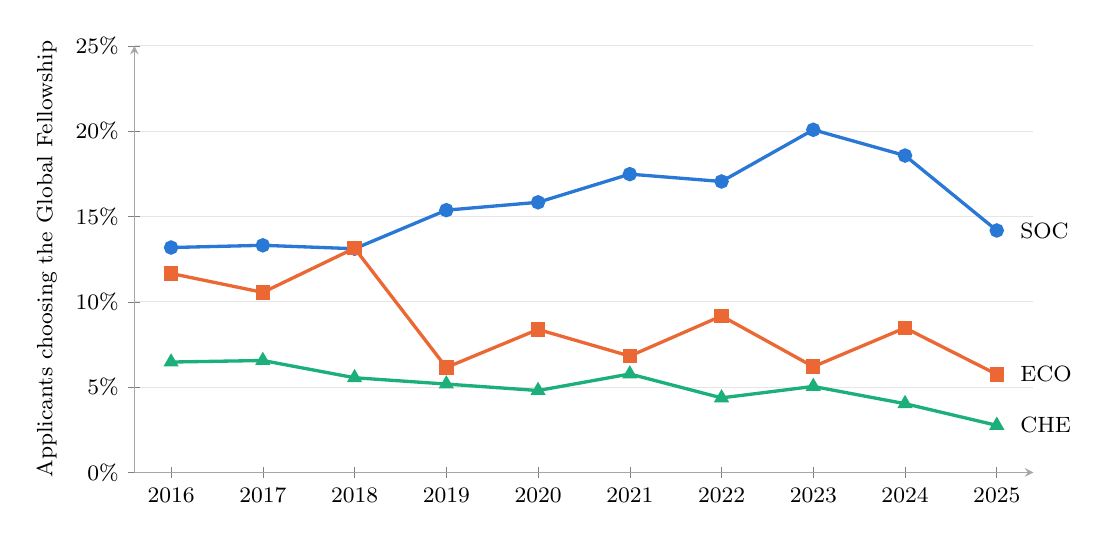
\begin{tikzpicture}
\begin{axis}[
  width=13cm, height=7cm,
  xmin=2015.6, xmax=2025.4, ymin=0, ymax=25,
  xtick={2016,2017,2018,2019,2020,2021,2022,2023,2024,2025}, xticklabel style={/pgf/number format/1000 sep={}},
  ytick distance=5, yticklabel={\pgfmathprintnumber{\tick}\%},
  axis x line=bottom, axis y line=left, axis line style={gray!70},
  ymajorgrids, grid style={gray!20},
  tick label style={font=\footnotesize}, label style={font=\footnotesize},
  ylabel={Applicants choosing the Global Fellowship},
  clip=false,
]
\addplot[color=mscaSOC, line width=1.2pt, mark=*, mark size=2pt] coordinates {(2016,13.18) (2017,13.31) (2018,13.11) (2019,15.37) (2020,15.83) (2021,17.48) (2022,17.05) (2023,20.08) (2024,18.57) (2025,14.18)};
\addplot[color=mscaECO, line width=1.2pt, mark=square*, mark size=2pt] coordinates {(2016,11.66) (2017,10.55) (2018,13.14) (2019,6.15) (2020,8.38) (2021,6.82) (2022,9.17) (2023,6.20) (2024,8.47) (2025,5.75)};
\addplot[color=mscaCHE, line width=1.2pt, mark=triangle*, mark size=2pt] coordinates {(2016,6.47) (2017,6.56) (2018,5.55) (2019,5.18) (2020,4.80) (2021,5.77) (2022,4.37) (2023,5.04) (2024,4.03) (2025,2.76)};
\node[font=\footnotesize, anchor=west] at (axis cs:2025.15,14.18) {SOC};
\node[font=\footnotesize, anchor=west] at (axis cs:2025.15,5.75) {ECO};
\node[font=\footnotesize, anchor=west] at (axis cs:2025.15,2.76) {CHE};
\end{axis}
\end{tikzpicture}
\caption{\footnotesize Share of eligible applicants to the Marie Sk\l{}odowska-Curie Actions postdoctoral
fellowships who applied to the Global rather than the European Fellowship, by panel, 2016--2025.
SOC: social sciences and humanities; ECO: economics; CHE: chemistry. Both EF and GF were introduced in 2014. However, 2016 is the earliest year where there is public data on application counts for each scientific field. In 2014 and 2015, field-specific application counts across all fields are not publicly available.}
\label{fig:msca_gf_share}
\end{figure}
